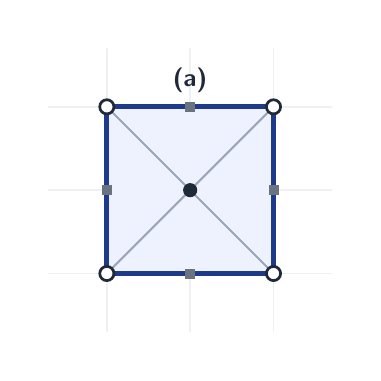
\begin{tikzpicture}[x=1bp, y=1bp]\path[use as bounding box] (0,0) rectangle (117.00,117.00);\clip (0,0) rectangle (117.00,117.00);
\path[draw={rgb,255:red,238;green,240;blue,243}, line width=0.52bp, line cap=round, line join=round] (28.50,7.50) -- (28.50,109.50);
\path[draw={rgb,255:red,238;green,240;blue,243}, line width=0.52bp, line cap=round, line join=round] (58.50,7.50) -- (58.50,109.50);
\path[draw={rgb,255:red,238;green,240;blue,243}, line width=0.52bp, line cap=round, line join=round] (88.50,7.50) -- (88.50,109.50);
\path[draw={rgb,255:red,238;green,240;blue,243}, line width=0.52bp, line cap=round, line join=round] (7.50,28.50) -- (109.50,28.50);
\path[draw={rgb,255:red,238;green,240;blue,243}, line width=0.52bp, line cap=round, line join=round] (7.50,58.50) -- (109.50,58.50);
\path[draw={rgb,255:red,238;green,240;blue,243}, line width=0.52bp, line cap=round, line join=round] (7.50,88.50) -- (109.50,88.50);
\path[fill={rgb,255:red,238;green,242;blue,255}] (28.50,28.50) rectangle (58.50,58.50);
\path[fill={rgb,255:red,238;green,242;blue,255}] (58.50,28.50) rectangle (88.50,58.50);
\path[fill={rgb,255:red,238;green,242;blue,255}] (28.50,58.50) rectangle (58.50,88.50);
\path[fill={rgb,255:red,238;green,242;blue,255}] (58.50,58.50) rectangle (88.50,88.50);
\path[draw={rgb,255:red,154;green,165;blue,184}, line width=0.60bp, line cap=round, line join=round] (58.50,58.50) -- (28.50,28.50);
\path[draw={rgb,255:red,154;green,165;blue,184}, line width=0.60bp, line cap=round, line join=round] (58.50,58.50) -- (28.50,28.50);
\path[draw={rgb,255:red,154;green,165;blue,184}, line width=0.60bp, line cap=round, line join=round] (58.50,58.50) -- (88.50,28.50);
\path[draw={rgb,255:red,154;green,165;blue,184}, line width=0.60bp, line cap=round, line join=round] (58.50,58.50) -- (88.50,28.50);
\path[draw={rgb,255:red,154;green,165;blue,184}, line width=0.60bp, line cap=round, line join=round] (58.50,58.50) -- (28.50,88.50);
\path[draw={rgb,255:red,154;green,165;blue,184}, line width=0.60bp, line cap=round, line join=round] (58.50,58.50) -- (28.50,88.50);
\path[draw={rgb,255:red,154;green,165;blue,184}, line width=0.60bp, line cap=round, line join=round] (58.50,58.50) -- (88.50,88.50);
\path[draw={rgb,255:red,154;green,165;blue,184}, line width=0.60bp, line cap=round, line join=round] (58.50,58.50) -- (88.50,88.50);
\path[draw={rgb,255:red,30;green,58;blue,138}, line width=1.80bp, line join=round] (28.50,28.50) -- (88.50,28.50) -- (88.50,88.50) -- (28.50,88.50) -- cycle;
\path[draw={rgb,255:red,31;green,41;blue,55}, line width=0.98bp, fill=white] (28.50,28.50) circle[radius=2.55bp];
\path[fill={rgb,255:red,107;green,114;blue,128}] (26.70,56.70) rectangle (30.30,60.30);
\path[draw={rgb,255:red,31;green,41;blue,55}, line width=0.98bp, fill=white] (28.50,88.50) circle[radius=2.55bp];
\path[fill={rgb,255:red,107;green,114;blue,128}] (56.70,26.70) rectangle (60.30,30.30);
\path[fill={rgb,255:red,31;green,41;blue,55}] (58.50,58.50) circle[radius=2.55bp];
\path[fill={rgb,255:red,107;green,114;blue,128}] (56.70,86.70) rectangle (60.30,90.30);
\path[draw={rgb,255:red,31;green,41;blue,55}, line width=0.98bp, fill=white] (88.50,28.50) circle[radius=2.55bp];
\path[fill={rgb,255:red,107;green,114;blue,128}] (86.70,56.70) rectangle (90.30,60.30);
\path[draw={rgb,255:red,31;green,41;blue,55}, line width=0.98bp, fill=white] (88.50,88.50) circle[radius=2.55bp];
\node[anchor=base, text={rgb,255:red,31;green,41;blue,55}, font=\fontsize{9.0}{10.8}\selectfont\sffamily\bfseries, inner sep=0pt] at (58.50,96.00) {(a)};
\end{tikzpicture}\hspace{27.0bp}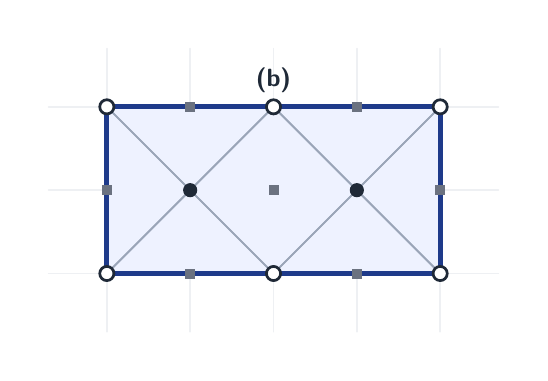
\begin{tikzpicture}[x=1bp, y=1bp]\path[use as bounding box] (0,0) rectangle (177.00,117.00);\clip (0,0) rectangle (177.00,117.00);
\path[draw={rgb,255:red,238;green,240;blue,243}, line width=0.52bp, line cap=round, line join=round] (28.50,7.50) -- (28.50,109.50);
\path[draw={rgb,255:red,238;green,240;blue,243}, line width=0.52bp, line cap=round, line join=round] (58.50,7.50) -- (58.50,109.50);
\path[draw={rgb,255:red,238;green,240;blue,243}, line width=0.52bp, line cap=round, line join=round] (88.50,7.50) -- (88.50,109.50);
\path[draw={rgb,255:red,238;green,240;blue,243}, line width=0.52bp, line cap=round, line join=round] (118.50,7.50) -- (118.50,109.50);
\path[draw={rgb,255:red,238;green,240;blue,243}, line width=0.52bp, line cap=round, line join=round] (148.50,7.50) -- (148.50,109.50);
\path[draw={rgb,255:red,238;green,240;blue,243}, line width=0.52bp, line cap=round, line join=round] (7.50,28.50) -- (169.50,28.50);
\path[draw={rgb,255:red,238;green,240;blue,243}, line width=0.52bp, line cap=round, line join=round] (7.50,58.50) -- (169.50,58.50);
\path[draw={rgb,255:red,238;green,240;blue,243}, line width=0.52bp, line cap=round, line join=round] (7.50,88.50) -- (169.50,88.50);
\path[fill={rgb,255:red,238;green,242;blue,255}] (28.50,28.50) rectangle (58.50,58.50);
\path[fill={rgb,255:red,238;green,242;blue,255}] (28.50,58.50) rectangle (58.50,88.50);
\path[fill={rgb,255:red,238;green,242;blue,255}] (58.50,28.50) rectangle (88.50,58.50);
\path[fill={rgb,255:red,238;green,242;blue,255}] (58.50,58.50) rectangle (88.50,88.50);
\path[fill={rgb,255:red,238;green,242;blue,255}] (88.50,28.50) rectangle (118.50,58.50);
\path[fill={rgb,255:red,238;green,242;blue,255}] (88.50,58.50) rectangle (118.50,88.50);
\path[fill={rgb,255:red,238;green,242;blue,255}] (118.50,28.50) rectangle (148.50,58.50);
\path[fill={rgb,255:red,238;green,242;blue,255}] (118.50,58.50) rectangle (148.50,88.50);
\path[draw={rgb,255:red,154;green,165;blue,184}, line width=0.60bp, line cap=round, line join=round] (58.50,58.50) -- (28.50,28.50);
\path[draw={rgb,255:red,154;green,165;blue,184}, line width=0.60bp, line cap=round, line join=round] (58.50,58.50) -- (28.50,28.50);
\path[draw={rgb,255:red,154;green,165;blue,184}, line width=0.60bp, line cap=round, line join=round] (58.50,58.50) -- (28.50,88.50);
\path[draw={rgb,255:red,154;green,165;blue,184}, line width=0.60bp, line cap=round, line join=round] (58.50,58.50) -- (28.50,88.50);
\path[draw={rgb,255:red,154;green,165;blue,184}, line width=0.60bp, line cap=round, line join=round] (58.50,58.50) -- (88.50,28.50);
\path[draw={rgb,255:red,154;green,165;blue,184}, line width=0.60bp, line cap=round, line join=round] (58.50,58.50) -- (88.50,28.50);
\path[draw={rgb,255:red,154;green,165;blue,184}, line width=0.60bp, line cap=round, line join=round] (58.50,58.50) -- (88.50,88.50);
\path[draw={rgb,255:red,154;green,165;blue,184}, line width=0.60bp, line cap=round, line join=round] (58.50,58.50) -- (88.50,88.50);
\path[draw={rgb,255:red,154;green,165;blue,184}, line width=0.60bp, line cap=round, line join=round] (118.50,58.50) -- (88.50,28.50);
\path[draw={rgb,255:red,154;green,165;blue,184}, line width=0.60bp, line cap=round, line join=round] (118.50,58.50) -- (88.50,28.50);
\path[draw={rgb,255:red,154;green,165;blue,184}, line width=0.60bp, line cap=round, line join=round] (118.50,58.50) -- (88.50,88.50);
\path[draw={rgb,255:red,154;green,165;blue,184}, line width=0.60bp, line cap=round, line join=round] (118.50,58.50) -- (88.50,88.50);
\path[draw={rgb,255:red,154;green,165;blue,184}, line width=0.60bp, line cap=round, line join=round] (118.50,58.50) -- (148.50,28.50);
\path[draw={rgb,255:red,154;green,165;blue,184}, line width=0.60bp, line cap=round, line join=round] (118.50,58.50) -- (148.50,28.50);
\path[draw={rgb,255:red,154;green,165;blue,184}, line width=0.60bp, line cap=round, line join=round] (118.50,58.50) -- (148.50,88.50);
\path[draw={rgb,255:red,154;green,165;blue,184}, line width=0.60bp, line cap=round, line join=round] (118.50,58.50) -- (148.50,88.50);
\path[draw={rgb,255:red,30;green,58;blue,138}, line width=1.80bp, line join=round] (28.50,28.50) -- (148.50,28.50) -- (148.50,88.50) -- (28.50,88.50) -- cycle;
\path[draw={rgb,255:red,31;green,41;blue,55}, line width=0.98bp, fill=white] (28.50,28.50) circle[radius=2.55bp];
\path[fill={rgb,255:red,107;green,114;blue,128}] (26.70,56.70) rectangle (30.30,60.30);
\path[draw={rgb,255:red,31;green,41;blue,55}, line width=0.98bp, fill=white] (28.50,88.50) circle[radius=2.55bp];
\path[fill={rgb,255:red,107;green,114;blue,128}] (56.70,26.70) rectangle (60.30,30.30);
\path[fill={rgb,255:red,31;green,41;blue,55}] (58.50,58.50) circle[radius=2.55bp];
\path[fill={rgb,255:red,107;green,114;blue,128}] (56.70,86.70) rectangle (60.30,90.30);
\path[draw={rgb,255:red,31;green,41;blue,55}, line width=0.98bp, fill=white] (88.50,28.50) circle[radius=2.55bp];
\path[fill={rgb,255:red,107;green,114;blue,128}] (86.70,56.70) rectangle (90.30,60.30);
\path[draw={rgb,255:red,31;green,41;blue,55}, line width=0.98bp, fill=white] (88.50,88.50) circle[radius=2.55bp];
\path[fill={rgb,255:red,107;green,114;blue,128}] (116.70,26.70) rectangle (120.30,30.30);
\path[fill={rgb,255:red,31;green,41;blue,55}] (118.50,58.50) circle[radius=2.55bp];
\path[fill={rgb,255:red,107;green,114;blue,128}] (116.70,86.70) rectangle (120.30,90.30);
\path[draw={rgb,255:red,31;green,41;blue,55}, line width=0.98bp, fill=white] (148.50,28.50) circle[radius=2.55bp];
\path[fill={rgb,255:red,107;green,114;blue,128}] (146.70,56.70) rectangle (150.30,60.30);
\path[draw={rgb,255:red,31;green,41;blue,55}, line width=0.98bp, fill=white] (148.50,88.50) circle[radius=2.55bp];
\node[anchor=base, text={rgb,255:red,31;green,41;blue,55}, font=\fontsize{9.0}{10.8}\selectfont\sffamily\bfseries, inner sep=0pt] at (88.50,96.00) {(b)};
\end{tikzpicture}
